\subsection{Histogram Processing}\label{sec:histogram-processing}

Et histogram i det vi har arbejdet med er en gengivelse af intensiteten i et billede. Figur~\ref{fig:hist-light}~til~\ref{fig:hist-high} viser eksempler på histogrammer for nogle billeder.

\begin{figure}[H]
	\centering
	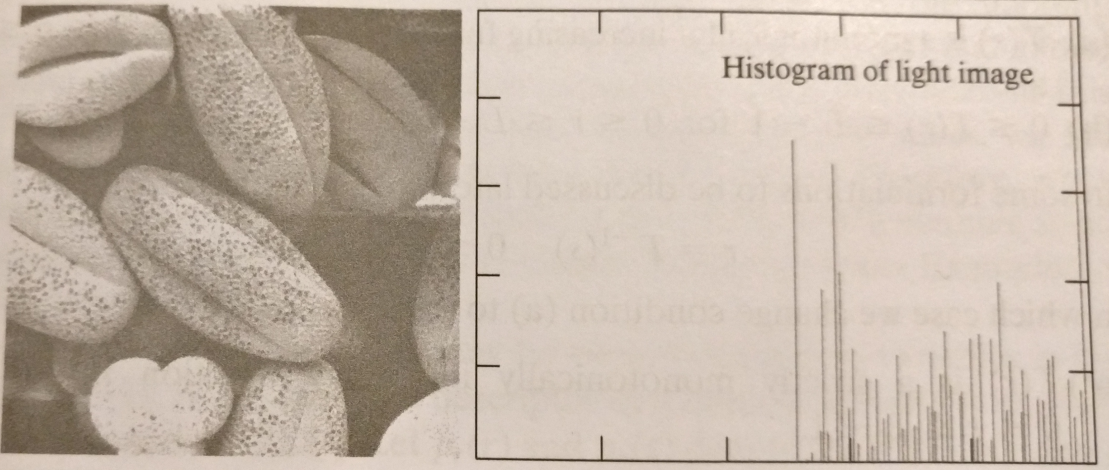
\includegraphics[width=0.6\linewidth]{figs/spm01/hist-light.png}
	\caption{Lyst billede.}
	\label{fig:hist-light}
\end{figure}

\begin{figure}[H]
	\centering
	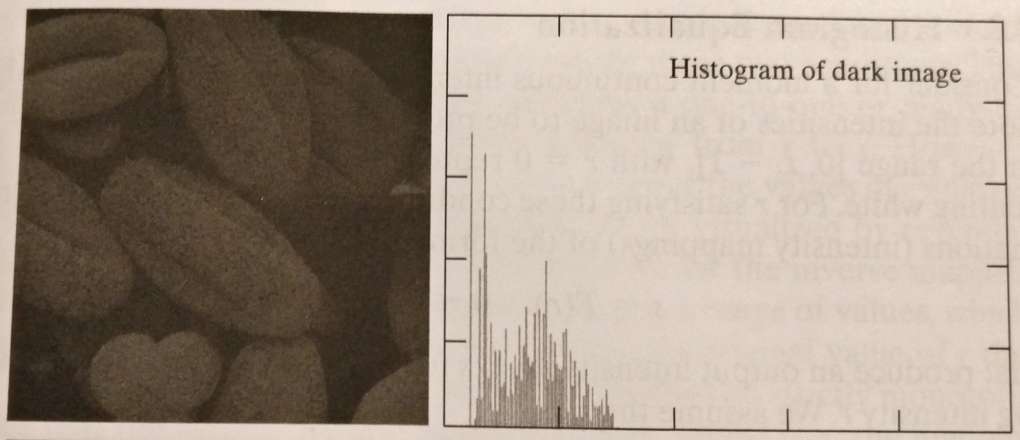
\includegraphics[width=0.6\linewidth]{figs/spm01/hist-dark.png}
	\caption{Mørkt billede.}
	\label{fig:hist-dark}
\end{figure}

\begin{figure}[H]
	\centering
	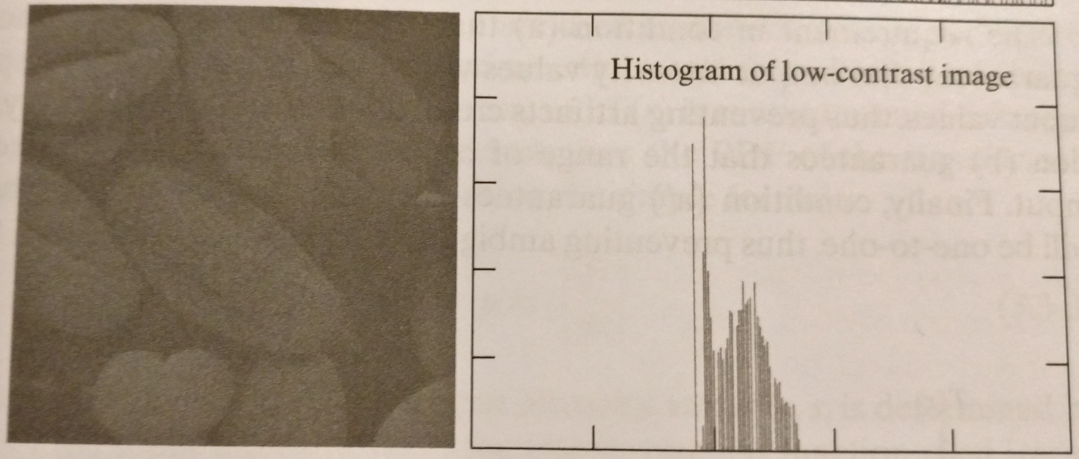
\includegraphics[width=0.6\linewidth]{figs/spm01/hist-low.png}
	\caption{Lav kontrast.}
	\label{fig:hist-low}
\end{figure}

\begin{figure}[H]
	\centering
	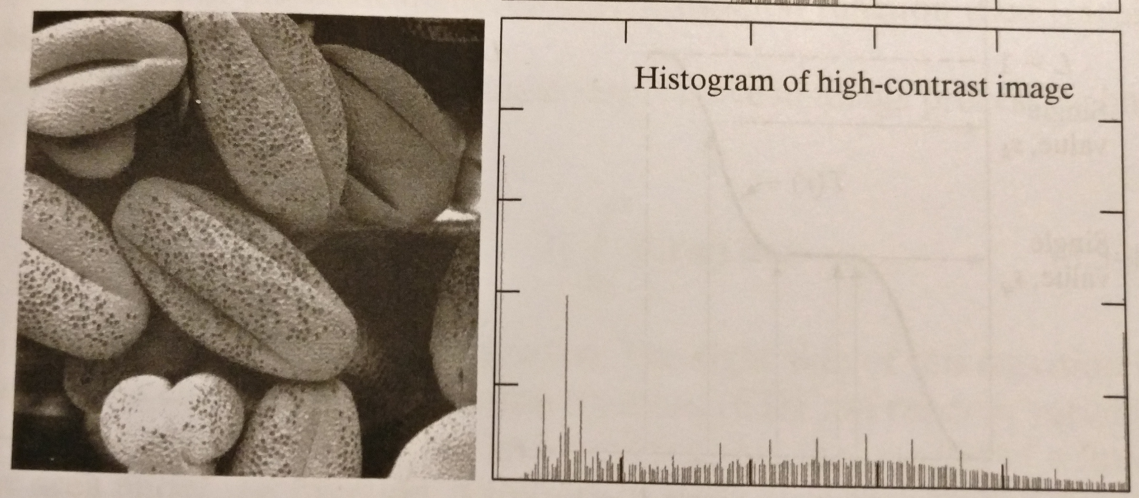
\includegraphics[width=0.6\linewidth]{figs/spm01/hist-high.png}
	\caption{Høj kontrast.}
	\label{fig:hist-high}
\end{figure}